\documentclass[a4paper,12pt]{article}
%%%%%%%%%%%%%%%%%%%%%%%%%%%%%%%%%%%%%%%%%%%%%%%%%%%%%%%%%%%%%%%%%%%%%%%%%%%%%%%%%%%%%%%%%%%%%%%%%%%%%%%%%%%%%%%%%%%%%%%%%%%%%%%%%%%%%%%%%%%%%%%%%%%%%%%%%%%%%%%%%%%%%%%%%%%%%%%%%%%%%%%%%%%%%%%%%%%%%%%%%%%%%%%%%%%%%%%%%%%%%%%%%%%%%%%%%%%%%%%%%%%%%%%%%%%%
\usepackage{eurosym}
\usepackage{vmargin}
\usepackage{amsmath}
\usepackage{graphics}
\usepackage{epsfig}
\usepackage{framed}
\usepackage{subfigure}
\usepackage{fancyhdr}

\setcounter{MaxMatrixCols}{10}
%TCIDATA{OutputFilter=LATEX.DLL}
%TCIDATA{Version=5.00.0.2570}
%TCIDATA{<META NAME="SaveForMode"CONTENT="1">}
%TCIDATA{LastRevised=Wednesday, February 23, 201113:24:34}
%TCIDATA{<META NAME="GraphicsSave" CONTENT="32">}
%TCIDATA{Language=American English}

\pagestyle{fancy}
\setmarginsrb{20mm}{0mm}{20mm}{25mm}{12mm}{11mm}{0mm}{11mm}
\lhead{MA4128} \rhead{Kevin O'Brien} \chead{Week 8} %\input{tcilatex}

%http://www.electronics.dit.ie/staff/ysemenova/Opto2/CO_IntroLab.pdf
\begin{document}
	
	\tableofcontents
	\newpage


\section{One-way MANOVA in SPSS}

\subsection{Introduction}
The one-way analysis of variance procedure (one-way ANOVA) is used to determine whether there are any differences between multiple independent groups on a continuous dependent variable. Suppose there was a study carried out on the mathematics results from three schools A, B and C. A one-way ANOVA procedure is used to test the hypothesis that the average score in each of the three schools is the same.
The alternative hypothesis is that the average score of one school is different to the others.
\begin{description}
\item[$H_0$] $\mu_A = \mu_B = \mu_C$
\item[$H_1$] There exists $\mu_i \neq \mu_j$ for some pairing of schools A B and C.
\end{description}
It is important to realize that the one-way ANOVA is an omnibus test statistic and cannot tell you which specific groups were significantly different from each other; it only tells you that at least two groups were different.

The one-way multivariate analysis of variance (one-way MANOVA) is used to determine whether there are any differences between independent groups on \textbf{more than one} continuous dependent variable. In this regard, it differs from a one-way ANOVA, which only measures one dependent variable.


For example, you could use a one-way MANOVA to understand whether there were differences in the perceptions of attractiveness and intelligence of drug users in movies (i.e., the two dependent variables are ``perceptions of attractiveness" and ``perceptions of intelligence", whilst the independent variable is ``drug users in movies", which has three independent groups: ``non-user", ``experimenter" and ``regular user").


Alternately, you could use a one-way MANOVA to understand whether there were differences in students' short-term and long-term recall of facts based on three different lengths of lecture (i.e., the two dependent variables are ``short-term memory recall" and ``long-term memory recall", whilst the independent variable is ``lecture duration", which has four independent groups: ``30 minutes", ``60 minutes", ``90 minutes" and ``120 minutes" , considered as categorical data, even though numeric data is valid also).

Again, it is important to realize that the one-way MANOVA is an omnibus test statistic and cannot tell you which specific groups were significantly different from each other; it only tells you that at least two groups were different. Since you may have three, four, five or more groups in your study design, determining which of these groups differ from each other is important. You can do this using a \textbf{post-hoc} test.


\subsection{Assumptions}
When you choose to analyze your data using a one-way MANOVA, part of the process involves checking to make sure that the data you want to analyze can actually be analyzed using a one-way MANOVA. You need to do this because it is only appropriate to use a one-way MANOVA if your data ``passes" nine assumptions that are required for a one-way MANOVA to give you a valid result. Do not be surprised if, when analyzing your own data using SPSS, one or more of these assumptions is violated. This is not uncommon when working with real-world data. However, even when your data fails certain assumptions, there is often a solution to overcome this.

In practice, checking for these nine Assumptions adds some more time to your analysis, requiring you to work through additional procedures in SPSS when performing your analysis, as well as thinking a little bit more about your data. These nine assumptions are presented below:

\begin{itemize}
\item \textbf{Assumption 1:} Your two or more dependent variables should be measured at the interval or ratio level (i.e., they are continuous). Examples of variables that meet this criterion include revision time (measured in hours), intelligence (measured using IQ score), exam performance (measured from 0 to 100), weight (measured in kg), and so forth.\\

\item \textbf{Assumption 2:} Your independent variable should consist of two or more categorical, independent groups. Example independent variables that meet this criterion include ethnicity (e.g., 3 groups: Caucasian, Afro-Caribbean and South Asian), physical activity level (e.g., 4 groups: sedentary, low, moderate and high), profession (e.g., 5 groups: surgeon, doctor, nurse, dentist, therapist), and so forth.\\

\item \textbf{Assumption 3:} You should have independence of observations, which means that there is no relationship between the observations in each group or between the groups themselves. For example, there must be different participants in each group with no participant being in more than one group. This is more of a study design issue than something you can test for, but it is an important assumption of the one-way MANOVA.\\

\item \textbf{Assumption 4:} You should have an adequate sample size. Although the larger your sample size, the better; for MANOVA, you need to have more cases in each group than the number of dependent variables you are analyzing.\\

\item \textbf{Assumption 5:} There are no univariate or multivariate outliers. First, there can be no (univariate) outliers in each group of the independent variable for any of the dependent variables. This is a similar assumption to the one-way ANOVA, but for each dependent variable that you have in your MANOVA analysis. Univariate outliers are often just called outliers and are the same type of outliers you will have come across if you have conducted t-tests or ANOVAs. We refer to them as univariate in this guide to distinguish them from multivariate outliers. Multivariate outliers are cases which have an unusual combination of scores on the dependent variables. \\ \smallskip


\begin{framed}Approaches for detecting outliers
    \begin{itemize} 
    \item[(1)] detect univariate outliers using boxplots,  
    \item[(2)] check for multivariate outliers using a measure called \textbf{Mahalanobis} distance.)
\end{itemize}
\end{framed}
\item \textbf{Assumption 6:} There is multivariate normality. Unfortunately, multivariate normality is a particularly tricky assumption to test for and cannot be directly tested in SPSS. Instead, normality of each of the dependent variables for each of the groups of the independent variable is often used in its place as a best 'guess' as to whether there is multivariate normality. You can test for this using the Shapiro-Wilk test of normality, which is easily tested for using SPSS. \\

\item \textbf{Assumption 7:} There is a linear relationship between each pair of dependent variables for each group of the independent variable. If the variables are not linearly related, the power of the test is reduced. You can test for this  assumption by plotting a scatterplot matrix for each group of the independent variable. In order to do this, you will need to split your data file in SPSS before generating the scatterplot matrices.
\item \textbf{Assumption 8:} There is a homogeneity of variance-covariance matrices. You can test this Assumption in SPSS using \textbf{Box's M test} of equality of covariance. If your data fails this assumption, you may also need to use SPSS to carry out \textbf{Levene's test} of homogeneity of variance to determine where the problem may lie.

\item \textbf{Assumption 9:} There is no multicollinearity. Ideally, you want your dependent variables to be moderately correlated with each other. If the correlations are low, you might be better off running separate one-way ANOVAs, and if the correlation(s) are too high (greater than 0.9), you could have multicollinearity. This is problematic for MANOVA and needs to be screened out.
\end{itemize}

You can check assumptions 5, 6, 7, 8 and 9 using SPSS. Before doing this, you should make sure that your data meets Assumptions 1, 2, 3 and 4, although you don't need SPSS to do this. Just remember that if you do not run the statistical tests on these assumptions correctly, the results you get when running a one-way MANOVA might not be valid.
\newpage

\subsection{Testing Assumptions with SPSS}
You can check assumptions 5, 6, 7, 8 and 9 using SPSS. Before doing this, you should make sure that your data meets Assumptions 1, 2, 3 and 4, although you don't need SPSS to do this. Just remember that if you do not run the statistical tests on these assumptions correctly, the results you get when running a one-way MANOVA might not be valid.
\newpage

\section{One-way MANOVA in SPSS}

\subsection{Introduction}
The one-way multivariate analysis of variance (one-way MANOVA) is used to determine whether there are any differences between independent groups on more than one continuous dependent variable. In this regard, it differs from a one-way ANOVA, which only measures one dependent variable. For example, you could use a one-way MANOVA to understand whether there were differences in the perceptions of attractiveness and intelligence of drug users in movies (i.e., the two dependent variables are "perceptions of attractiveness" and "perceptions of intelligence", whilst the independent variable is "drug users in movies", which has three independent groups: "non-user", "experimenter" and "regular user"). Alternately, you could use a one-way MANOVA to understand whether there were differences in students' short-term and long-term recall of facts based on three different lengths of lecture (i.e., the two dependent variables are "short-term memory recall" and "long-term memory recall", whilst the independent variable is "lecture duration", which has four independent groups: "30 minutes", "60 minutes", "90 minutes" and "120 minutes").

It is important to realise that the one-way MANOVA is an omnibus test statistic and cannot tell you which specific groups were significantly different from each other; it only tells you that at least two groups were different. Since you may have three, four, five or more groups in your study design, determining which of these groups differ from each other is important. You can do this using a post-hoc test (N.B., we discuss post-hoc tests later in this guide).

In this "quick start" guide, we show you how to carry out a one-way MANOVA using SPSS, as well as interpret and report the results from this test. Since the one-way MANOVA is often followed up with post-hoc tests, we also show you how to carry these out using SPSS. However, before we introduce you to this procedure, you need to understand the different assumptions that your data must meet in order for a one-way MANOVA to give you a valid result. We discuss these  Assumptions next.



\subsection{Example}
The pupils at a high school come from three different primary schools. The headteacher wanted to know whether there were academic differences between the pupils from the three different primary schools. As such, she randomly selected 20 pupils from School A, 20 pupils from School B and 20 pupils from School C, and measured their academic performance as assessed by the marks they received for their end-of-year English and Maths exams. Therefore, the two dependent variables were ``English score" and ``Maths score", whilst the independent variable was ``School", which consisted of three categories: ``School A", ``School B" and ``School C".



\subsection{Setup in SPSS}
In SPSS, we separated the groups for analysis by creating a grouping variable called School (i.e., the independent variable), and gave the three categories of the independent variable the labels $School A$, $School B$ and $School C$. The two dependent variables were labelled $English_Score$ and $Maths_Score$, respectively. It is also recommended that you create a fourth variable, $subject_id$, to act as a case number. This latter variable is required to test whether there are any multivariate outliers (i.e., part of Assumption 5 above).

%However, in the one-way MANOVA guide, we show you how to correctly enter data in SPSS to run a one-way MANOVA when you are also checking for assumptions. You can learn about our  data setup content here. Alternately, we have a generic, "quick start" guide to show you how to enter data into SPSS, available here.

%============================================================%


\subsection{Test Procedure in SPSS}
The following steps below show you how to analyse your data using a one-way MANOVA in SPSS when the nine assumptions in the previous section, ssumptions, have not been violated. At the end of these 14 steps, we show you how to interpret the results from this test.
\begin{verbatim}
Click Analyze > General Linear Model > Multivariate
\end{verbatim}
on the top menu as shown below:



You will be presented with the Multivariate dialogue box:

\begin{center}
	\begin{figure}[h!]
		% Requires \usepackage{graphicx}
		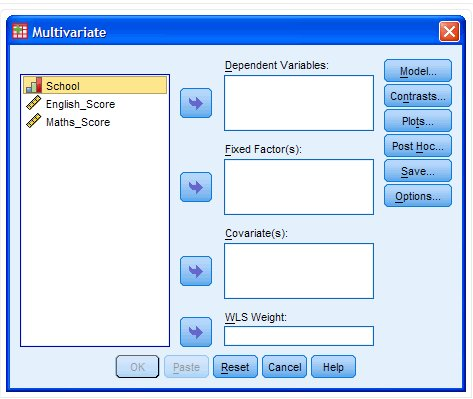
\includegraphics[scale=0.4]{MANOVA1}\\
		\caption{MANOVA}
	\end{figure}
\end{center}

%Transfer the independent variable, School, into the \texttt{Fixed Factor(s):} box and transfer the dependent variables, English Score and Maths Score, into the
%\texttt{Dependent Variables: box.} You can do this by drag-and-dropping the variables into their respective boxes or by using the  button.
%
%\begin{center}
%\begin{figure}[h!]
%  % Requires \usepackage{graphicx}
%  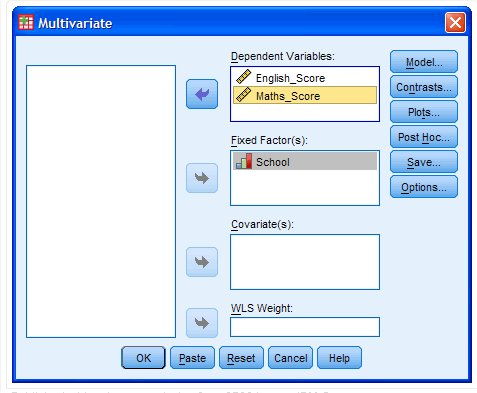
\includegraphics[scale=0.4]{MANOVA2}\\
%  \caption{MANOVA}
%\end{figure}
%\end{center}
%
%(Note: For this analysis, you will not need to use the Covariate(s): box (used for MANCOVA) or the WLS Weight: box.)
%
%Click on the  button. You will be presented with the Multivariate: Profile Plots dialogue box:
%
%
%\begin{center}
%\begin{figure}[h!]
%  % Requires \usepackage{graphicx}
%  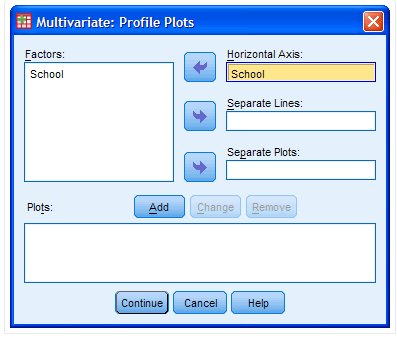
\includegraphics[scale=0.4]{MANOVA3}\\
%  \caption{MANOVA}
%\end{figure}
%\end{center}
%Transfer the independent variable, School, into the Horizontal Axis: box.
%
%
%Click the  button. You will see that "School" has been added to the Plots: box.
%
%
%Click the  button. This will return you to the Multivariate dialogue box.
%
%Click the  button. You will be presented with the Multivariate: Post Hoc Multiple Comparisons for Observed... dialogue box.
%
%\begin{center}
%\begin{figure}[h!]
%  % Requires \usepackage{graphicx}
%  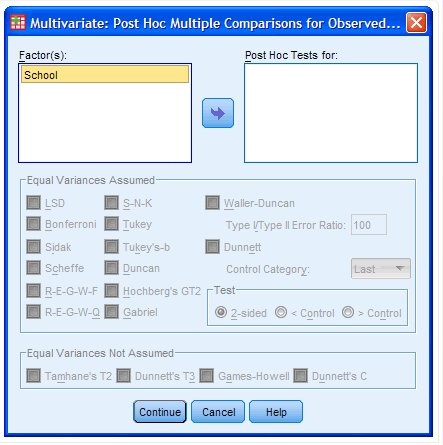
\includegraphics[scale=0.4]{MANOVA4}\\
%  \caption{MANOVA}
%\end{figure}
%\end{center}
%
%Transfer the independent variable, School, into the Post Hoc Tests for: box and select the Tukey checkbox in the -Equal Variances Assumed- area.
%
%
%\begin{center}
%\begin{figure}[h!]
%  % Requires \usepackage{graphicx}
%  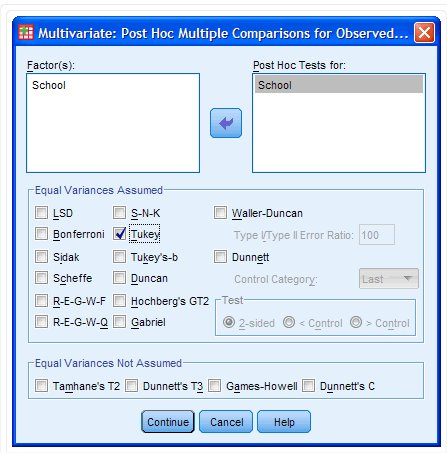
\includegraphics[scale=0.4]{MANOVA5}\\
%  \caption{MANOVA}
%\end{figure}
%\end{center}
%
%Note: You can select other post-hoc tests depending on your data and study design. If your independent variable only has two levels/categories, you do not need to complete this post-hoc section.
%
%Click the  button. This will return you to the Multivariate dialogue box.
%
%
%Click the  button. This will present you with the Multivariate: Options dialogue box.
%
%
%Transfer the independent variable, "School", from the Factor(s) and Factor Interactions: box into the Display Means for: box. Select the Descriptive statistics, Estimates of effect size and Observed power checkboxes in the -Display- area. You will be presented with the following screen:
%
%\begin{center}
%\begin{figure}[h!]
%  % Requires \usepackage{graphicx}
%  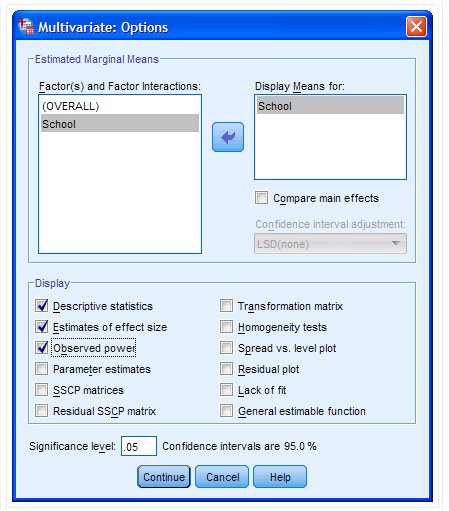
\includegraphics[scale=0.4]{MANOVA6}\\
%  \caption{MANOVA}
%\end{figure}
%\end{center}


\subsection{SPSS Output of the One-Way MANOVA}
\begin{itemize}
	\item SPSS produces many different tables in its one-way MANOVA analysis. In this section, we show you only the main tables required to understand your results from the one-way MANOVA and Tukey post-hoc tests. For a complete explanation of the output you have to interpret when checking your data for the nine assumptions required to carry out a one-way MANOVA. 
	
	\item This includes relevant boxplots, scatterplot matrix and Pearson's correlation coefficients, and output from your Mahalanobis distance test, Shapiro-Wilk test for normality, and Box's M test of equality of covariance, and if required, Levene's test of homogeneity of variance.
	
	\item However, the emphasis will be placed on the four main tables you need to understandthe one-way MANOVA results, assuming that your data has already met the nine assumptions required for a one-way MANOVA to give you a valid result.
\end{itemize}




\subsection{Descriptive Statistics}
The first important one is the Descriptive Statistics table. This table is very useful as it provides the mean and standard deviation for the two different dependent variables, which have been split by the independent variable. In addition, the table provides "Total" rows, which allows means and standard deviations for groups only split by the dependent variable to be known.

\begin{center}
	\begin{figure}[h!]
		% Requires \usepackage{graphicx}
		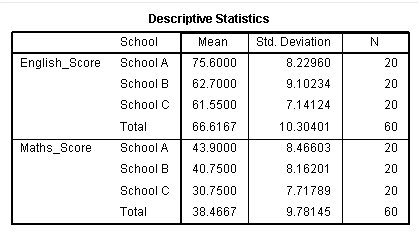
\includegraphics[scale=0.6]{MANOVA8}\\
		\caption{MANOVA}
	\end{figure}
\end{center}






\subsection{Multivariate Tests}
The Multivariate Tests table is where we find the actual result of the one-way MANOVA. You need to look at the second Effect, labelled "School", and the Wilks' Lambda row (highlighted in red). To determine whether the one-way MANOVA was statistically significant you need to look at the \textbf{Sig.} column. We can see from the table that we have a "Sig." value of .000, which means $p < .0005$. Therefore, we can conclude that this school's pupils academic performance was significantly dependent on which prior school they had attended ($p < .0005$).


\begin{center}
	\begin{figure}[h!]
		% Requires \usepackage{graphicx}
		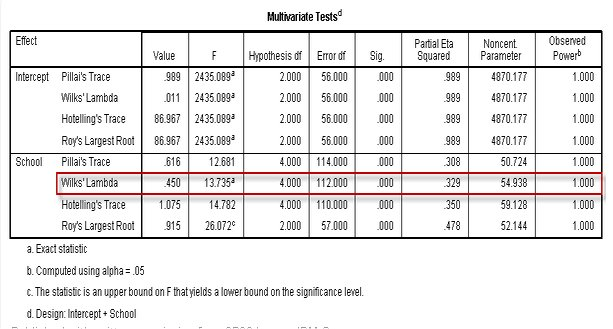
\includegraphics[scale=0.6]{MANOVA7}\\
		\caption{MANOVA}
	\end{figure}
\end{center}





\subsection{Reporting the Result (without follow-up tests)}
You could report the result of this test as follows:

\emph{
	There was a statistically significant difference in academic performance based on a pupil's prior school , $F(4, 112) = 13.74$, $p < .0005$; Wilk's Lambda = 0.450, partial $\eta^2$ = 0.33.
}

If you had not achieved a statistically significant result, you would not perform any further follow-up tests. However, as our case shows that we did, we will continue with further tests.







\subsection{Reporting the Result (without follow-up tests)}
You could report the result of this test as follows:

\subsubsection{General}
There was a statistically significant difference in academic performance based on a pupil's prior school , F (4, 112) = 13.74, $p < .0005$; Wilk's Lambda = 0.450, partial $\eta^2$ = 0.33.

If you had not achieved a statistically significant result, you would not perform any further follow-up tests. However, as our case shows that we did, we will continue with further tests.





\subsection{Univariate ANOVAs}
To determine how the dependent variables differ for the independent variable, we need to look at the Tests of Between-Subjects Effects table (highlighted in red):

\begin{center}
	\begin{figure}[h!]
		% Requires \usepackage{graphicx}
		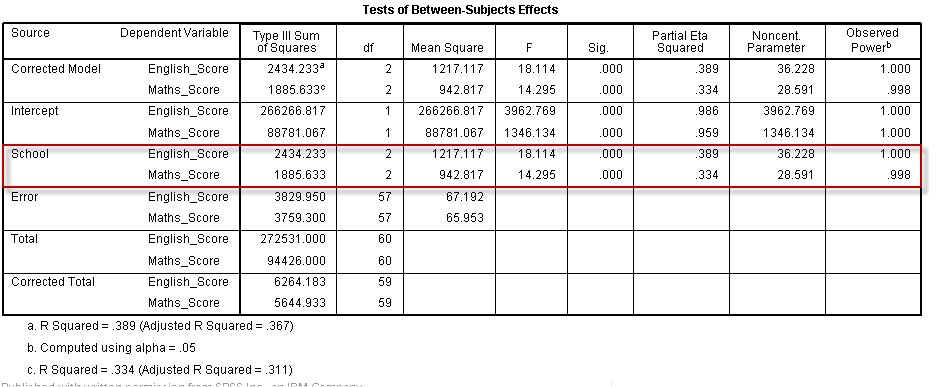
\includegraphics[scale=0.5]{MANOVA9}\\
		\caption{MANOVA}
	\end{figure}
\end{center}

We can see from this table that prior schooling has a statistically significant effect on both English $(F (2, 57) = 18.11$; $p < .0005$; partial $\eta^2$ $= .39)$ and Maths scores $(F (2, 57) = 14.30$; $p < .0005$; partial $\eta^2$ = .33).
(It is important to note that, in practice, you should make an \textbf{alpha correction} to account for multiple ANOVAs being run, such as a Bonferroni correction. As such, in this case, we accept statistical significance at p < .025.)





\subsection{Multiple Comparisons}
We can follow up these significant ANOVAs with Tukey's HSD post-hoc tests, as shown below in the Multiple Comparisons table:

\begin{center}
	\begin{figure}[h!]
		% Requires \usepackage{graphicx}
		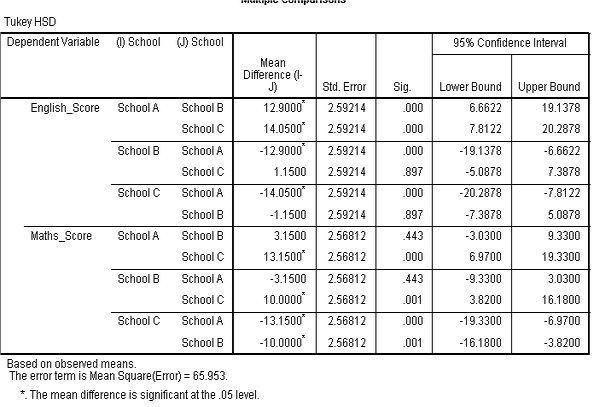
\includegraphics[scale=0.6]{MANOVA10}\\
		\caption{MANOVA}
	\end{figure}
\end{center}

The table above shows that for mean scores for English were statistically significantly different between School A and School B ($p < .0005$), and School A and School C ($p < .0005$), but not between School B and School C (p = .897). Mean maths scores were statistically significantly different between School A and School C ($p < .0005$), and School B and School C (p = .001), but not between School A and School B (p = .443). These differences can be easily visualised by the plots generated by this procedure, as shown below:

\begin{center}
	\begin{figure}[h!]
		% Requires \usepackage{graphicx}
		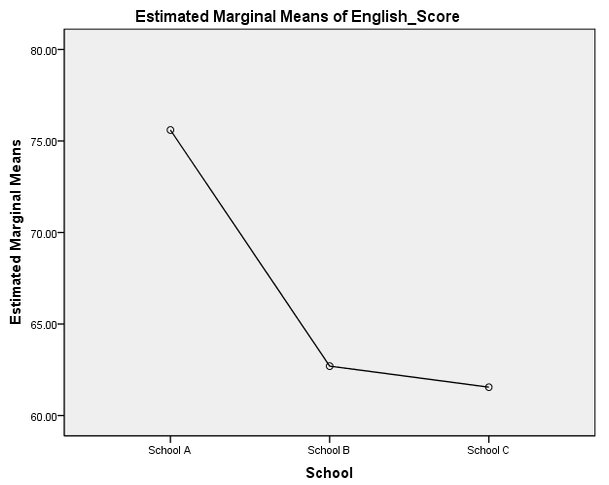
\includegraphics[scale=0.4]{MANOVA11}\\
		\caption{MANOVA}
	\end{figure}
\end{center}
\begin{center}
	\begin{figure}[h!]
		% Requires \usepackage{graphicx}
		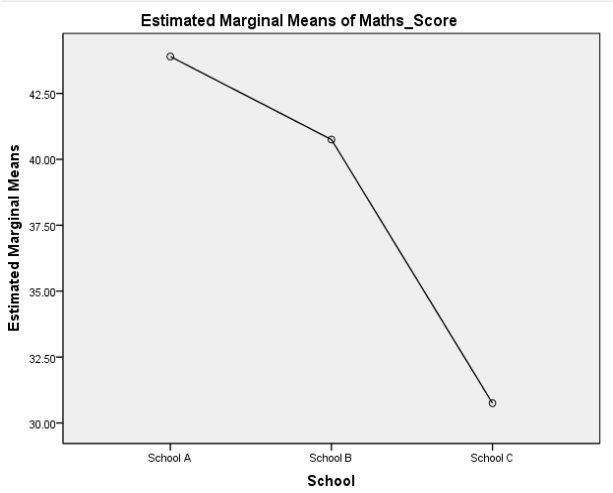
\includegraphics[scale=0.4]{MANOVA12}\\
		\caption{MANOVA}
	\end{figure}
\end{center}


\subsection{Multiple Comparisons}
We can follow up these significant ANOVAs with Tukey's HSD post-hoc tests, as shown below in the Multiple Comparisons table:

\begin{center}
	\begin{figure}[h!]
		% Requires \usepackage{graphicx}
		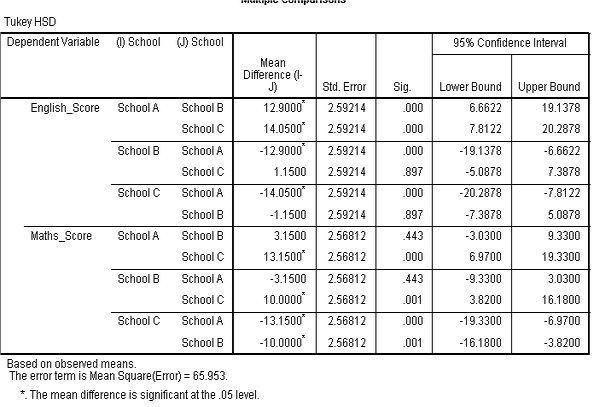
\includegraphics[scale=0.6]{MANOVA10}\\
		\caption{MANOVA}
	\end{figure}
\end{center}

The table above shows that for mean scores for English were statistically significantly different between School A and School B ($p < .0005$), and School A and School C ($p < .0005$), but not between School B and School C (p = .897). Mean maths scores were statistically significantly different between School A and School C ($p < .0005$), and School B and School C (p = .001), but not between School A and School B (p = .443). These differences can be easily visualised by the plots generated by this procedure, as shown below:

\begin{center}
	\begin{figure}[h!]
		% Requires \usepackage{graphicx}
		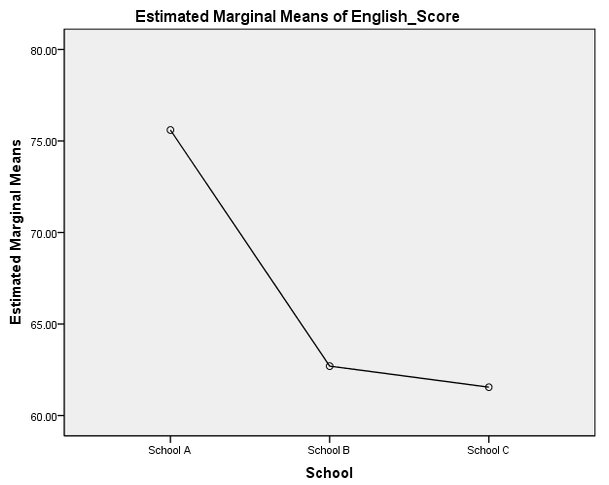
\includegraphics[scale=0.4]{MANOVA11}\\
		\caption{MANOVA}
	\end{figure}
\end{center}
\begin{center}
	\begin{figure}[h!]
		% Requires \usepackage{graphicx}
		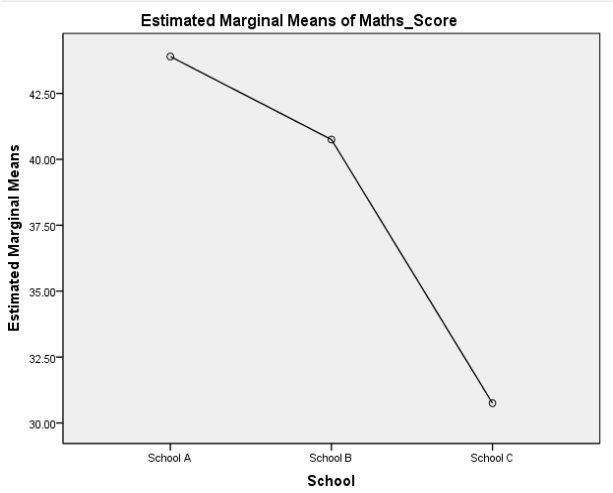
\includegraphics[scale=0.4]{MANOVA12}\\
		\caption{MANOVA}
	\end{figure}
\end{center}






\section{Implementation}
In the section,we will illustrate the SPSS procedure to perform a one-way MANOVA assuming that no assumptions have been violated. First, we set out the example we use to explain the one-way MANOVA procedure in SPSS.



\subsection{Example}
The pupils at a high school come from three different primary schools. The headteacher wanted to know whether there were academic differences between the pupils from the three different primary schools. As such, she randomly selected 20 pupils from School A, 20 pupils from School B and 20 pupils from School C, and measured their academic performance as assessed by the marks they received for their end-of-year English and Maths exams. Therefore, the two dependent variables were ``English score" and ``Maths score", whilst the independent variable was ``School", which consisted of three categories: ``School A", ``School B" and ``School C".





\subsection{Test Procedure in SPSS}
The following steps below show you how to analyse your data using a one-way MANOVA in SPSS when the nine assumptions in the previous section, ssumptions, have not been violated. At the end of these 14 steps, we show you how to interpret the results from this test.
\begin{verbatim}
Click Analyze > General Linear Model > Multivariate
\end{verbatim}
on the top menu as shown below:



You will be presented with the Multivariate dialogue box:

\begin{center}
	\begin{figure}[h!]
		% Requires \usepackage{graphicx}
		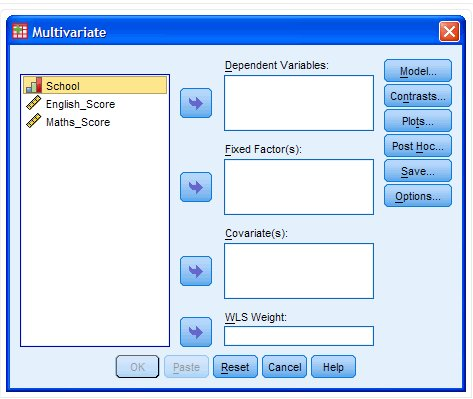
\includegraphics[scale=0.4]{MANOVA1}\\
		\caption{MANOVA}
	\end{figure}
\end{center}

%Transfer the independent variable, School, into the \texttt{Fixed Factor(s):} box and transfer the dependent variables, English Score and Maths Score, into the
%\texttt{Dependent Variables: box.} You can do this by drag-and-dropping the variables into their respective boxes or by using the  button.
%
%\begin{center}
%\begin{figure}[h!]
%  % Requires \usepackage{graphicx}
%  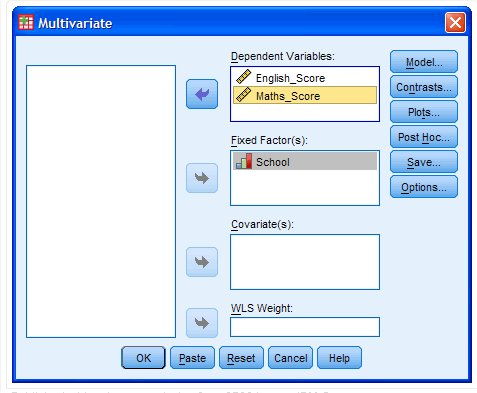
\includegraphics[scale=0.4]{MANOVA2}\\
%  \caption{MANOVA}
%\end{figure}
%\end{center}
%
%(Note: For this analysis, you will not need to use the Covariate(s): box (used for MANCOVA) or the WLS Weight: box.)
%
%Click on the  button. You will be presented with the Multivariate: Profile Plots dialogue box:
%
%
%\begin{center}
%\begin{figure}[h!]
%  % Requires \usepackage{graphicx}
%  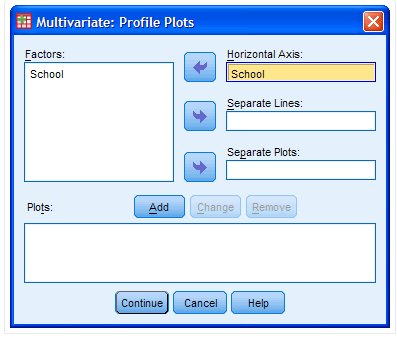
\includegraphics[scale=0.4]{MANOVA3}\\
%  \caption{MANOVA}
%\end{figure}
%\end{center}
%Transfer the independent variable, School, into the Horizontal Axis: box.
%
%
%Click the  button. You will see that "School" has been added to the Plots: box.
%
%
%Click the  button. This will return you to the Multivariate dialogue box.
%
%Click the  button. You will be presented with the Multivariate: Post Hoc Multiple Comparisons for Observed... dialogue box.
%
%\begin{center}
%\begin{figure}[h!]
%  % Requires \usepackage{graphicx}
%  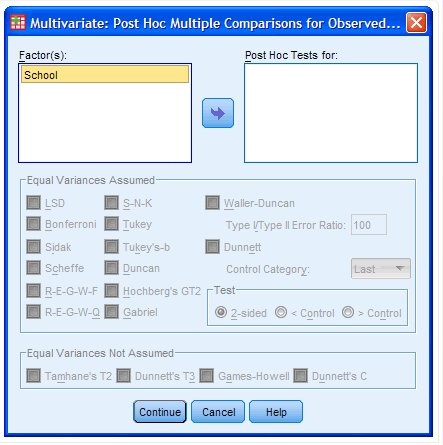
\includegraphics[scale=0.4]{MANOVA4}\\
%  \caption{MANOVA}
%\end{figure}
%\end{center}
%
%Transfer the independent variable, School, into the Post Hoc Tests for: box and select the Tukey checkbox in the -Equal Variances Assumed- area.
%
%
%\begin{center}
%\begin{figure}[h!]
%  % Requires \usepackage{graphicx}
%  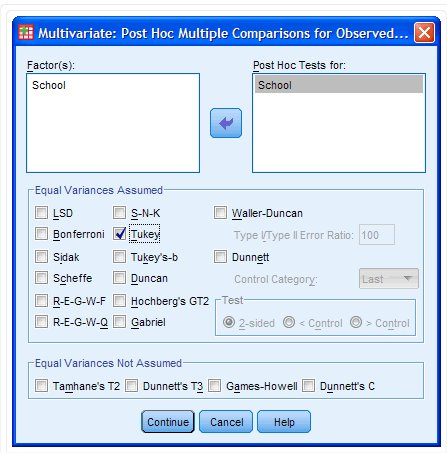
\includegraphics[scale=0.4]{MANOVA5}\\
%  \caption{MANOVA}
%\end{figure}
%\end{center}
%
%Note: You can select other post-hoc tests depending on your data and study design. If your independent variable only has two levels/categories, you do not need to complete this post-hoc section.
%
%Click the  button. This will return you to the Multivariate dialogue box.
%
%
%Click the  button. This will present you with the Multivariate: Options dialogue box.
%
%
%Transfer the independent variable, "School", from the Factor(s) and Factor Interactions: box into the Display Means for: box. Select the Descriptive statistics, Estimates of effect size and Observed power checkboxes in the -Display- area. You will be presented with the following screen:
%
%\begin{center}
%\begin{figure}[h!]
%  % Requires \usepackage{graphicx}
%  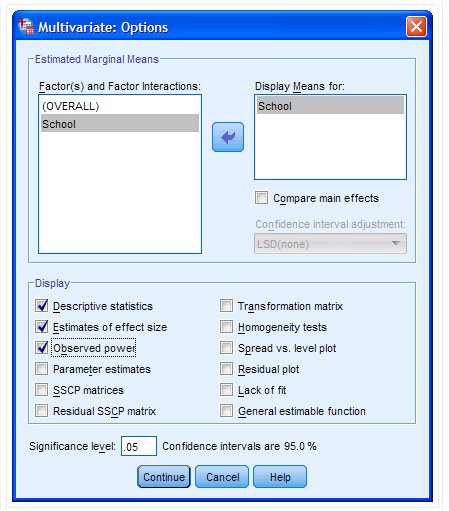
\includegraphics[scale=0.4]{MANOVA6}\\
%  \caption{MANOVA}
%\end{figure}
%\end{center}
%
%
%Click the  button. This will return you to the Multivariate dialogue box.
%
%Click the  button to generate the output.
\newpage
\section{SPSS Output of the One-Way MANOVA}
SPSS produces many different tables in its one-way MANOVA analysis. In this section, we show you only the main tables required to understand your results from the one-way MANOVA and Tukey post-hoc tests.

\begin{quote}
	For a complete explanation of the output you have to interpret when checking your data for the nine assumptions required to carry out a one-way MANOVA.
	
	This includes relevant boxplots, scatterplot matrix and Pearson's correlation coefficients, and output from your Mahalanobis distance test, Shapiro-Wilk test for normality, and Box's M test of equality of covariance, and if required, Levene's test of homogeneity of variance.
\end{quote}
However, the emphasis will be placed on the four main tables you need to understandthe one-way MANOVA results, assuming that your data has already met the nine assumptions required for a one-way MANOVA to give you a valid result.







\section{Implementation}
In the section,we will illustrate the SPSS procedure to perform a one-way MANOVA assuming that no assumptions have been violated. First, we set out the example we use to explain the one-way MANOVA procedure in SPSS.




\subsection{SPSS Output of the One-Way MANOVA}
SPSS produces many different tables in its one-way MANOVA analysis. In this section, we show you only the main tables required to understand your results from the one-way MANOVA and Tukey post-hoc tests.

\begin{quote}
For a complete explanation of the output you have to interpret when checking your data for the nine assumptions required to carry out a one-way MANOVA.

This includes relevant boxplots, scatterplot matrix and Pearson's correlation coefficients, and output from your Mahalanobis distance test, Shapiro-Wilk test for normality, and Box's M test of equality of covariance, and if required, Levene's test of homogeneity of variance.
\end{quote}
However, the emphasis will be placed on the four main tables you need to understandthe one-way MANOVA results, assuming that your data has already met the nine assumptions required for a one-way MANOVA to give you a valid result.






\end{document} 